\documentclass[handout]{beamer}
\usepackage{ulem}
\usepackage{multirow}

\usetheme{Warsaw}
%\usecolortheme{seahorse}

%Information to be included in the title page:
\title %optional
{SignNet: Recognize Alphabets in the American Sign Language in Real Time}

\author[Zeqiang, Kexiang, Zhiyuan] % (optional, for multiple authors)
{Zeqiang Lai \and Kexiang Huang \and Zhiyuan Liang}

\institute[BIT] % (optional)
{
  School of Computer Science\\
  Beijing Institute of Technology
}

\date[CV 2020] % (optional)
{Course of Computer Vision, December 2020}



\begin{document}

\frame{\titlepage}

\begin{frame}[t]{Introduction}

\begin{columns}
\column{0.5\textwidth}
\begin{itemize}
	\item Sign Language Recognition
	\item 26 Letters \&\& Space, Delete
	\item Real Time Demo with Common Commercial Camera
\end{itemize}

\column{0.5\textwidth}
\begin{figure}
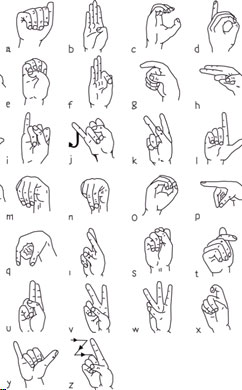
\includegraphics[scale=0.4]{imgs/NIDCD-ASL-hands-2014}
\caption{American Sign Language}
\end{figure}

\end{columns}


\end{frame}


\begin{frame}
\frametitle{Approach}

\begin{enumerate}
	\item Formulate the task as an \textbf{image classification} problem.
	\pause
	\item Use a modified version of \textbf{VGG} network for recogniton.
	\pause
	\item Trained on the \textbf{custom dataset} collected by our own.
\end{enumerate}

\end{frame}

\begin{frame}
\frametitle{Modified VGG}

\begin{figure}
\begin{center}
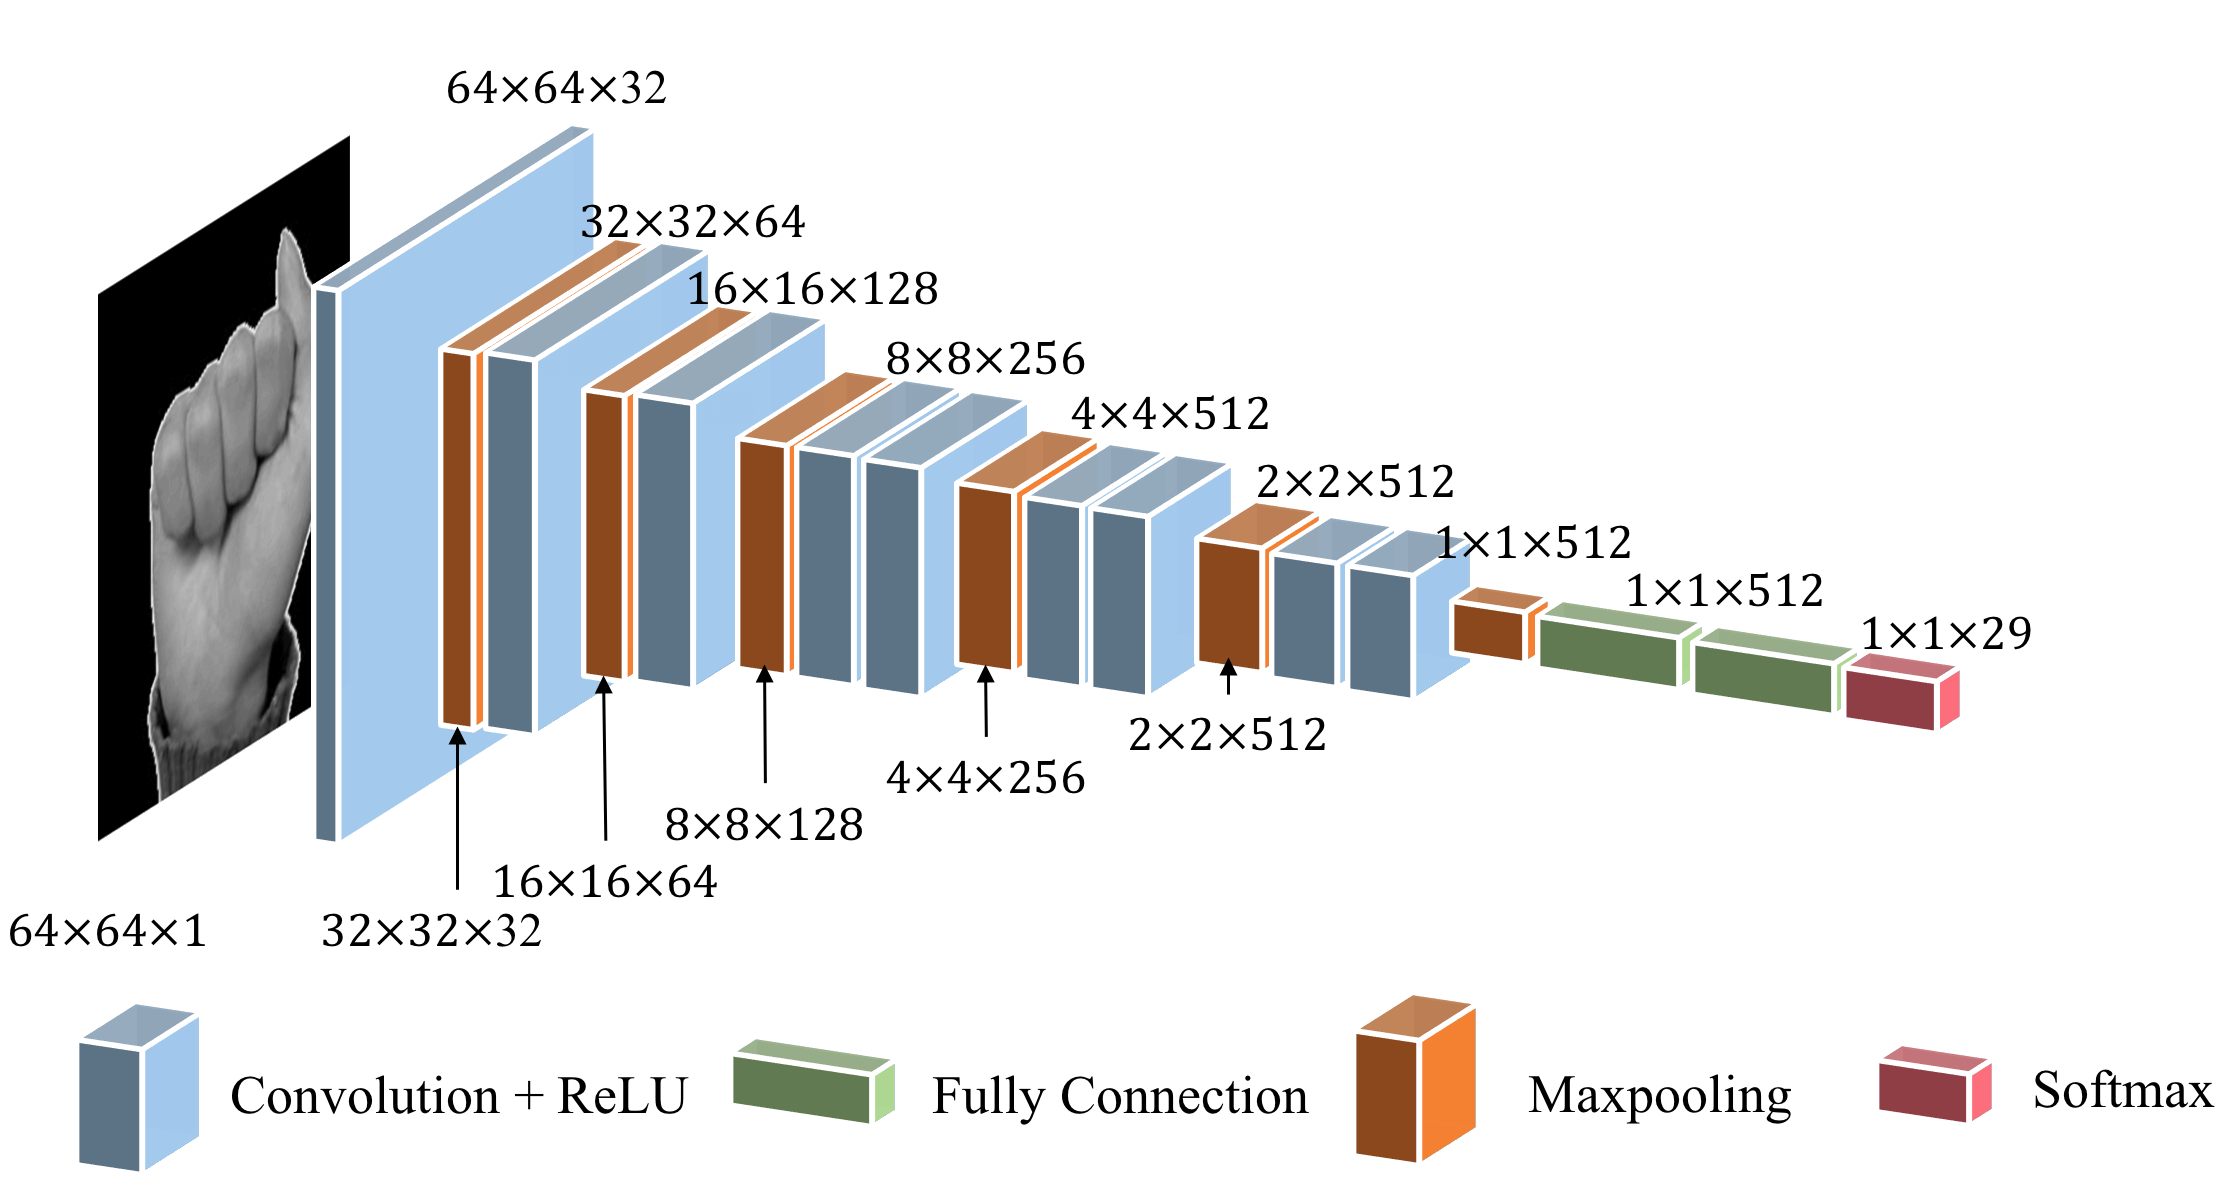
\includegraphics[scale=0.13]{imgs/arch}
\end{center}
\caption{Network architecture}
\end{figure}

\end{frame}


\begin{frame}
\frametitle{First Try: Train on ASL Dataset}

\begin{enumerate}
	\item<+-| structure@+> ASL Alphabet is a public available dataset
	\begin{itemize}
		\item 200 $\times$ 200 color image.
		\item Training set contains 87000 images (29 classes, 3000 for each class).
		\item Test set contains 870 images, 300 for each class.
	\end{itemize}
	\item<+-| structure@+> Train with origin pictures firstly (Bad performance)
	\item<+-| structure@+> Train with cropped - gaussian blurred - grayscale version (Still Bad)
\end{enumerate}

\end{frame}

\begin{frame}
\frametitle{First Try: ASL Result}

\begin{table}[h]
\begin{center}
\begin{tabular}{|l|c|}
\hline
Dataset & Accuracy \\
\hline\hline
ASL Alphabet Train & 86906/87000 (100\%) \\
ASL Alphabet Test & 145/870 (17\%) \\
Our ASL Test Set & 1087/21418 (5\%) \\
\hline
\end{tabular}
\end{center}
\caption{Results on ASL dataset.}
\label{table:result}
\end{table}

\end{frame}

\begin{frame}
\frametitle{Analysis}

\begin{block}

Why our model works perfectly on training set, but fails on test set ?

\end{block}

\
\

\begin{itemize}
	\item Obviously, \textbf{Overfit!}
	\item Training set lacks variation on the background.

\end{itemize}

\end{frame}

\begin{frame}
\frametitle{Analysis}

\begin{figure}[h]
\begin{center}
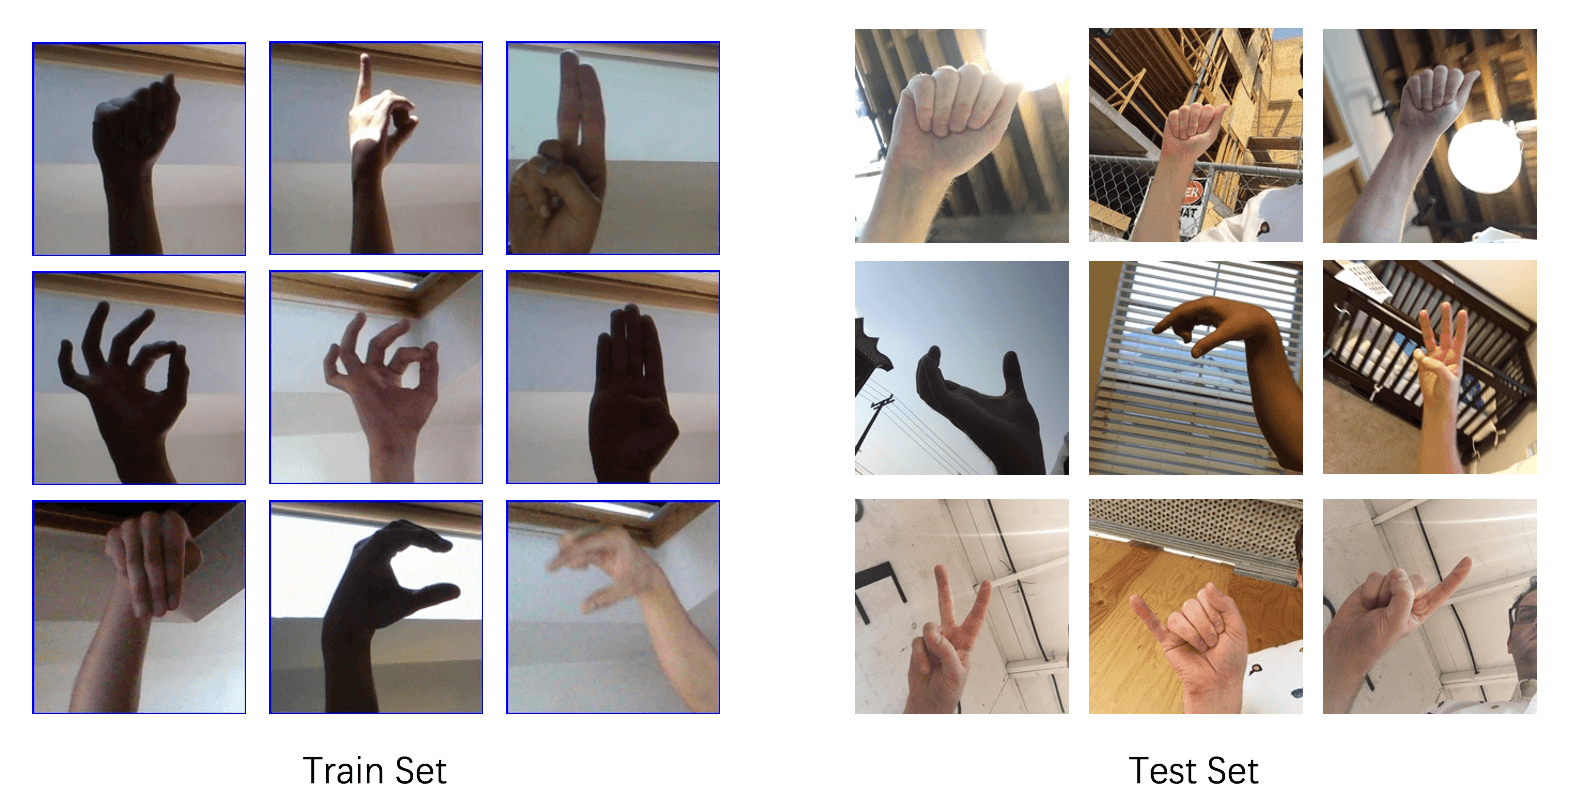
\includegraphics[width=1\linewidth]{imgs/asl-cmp}
\end{center}
\end{figure}

\end{frame}

\begin{frame}
\frametitle{Improvement}

\begin{itemize}
	\item Record dataset with diverse backgrounds ?
\end{itemize}

\end{frame}

\begin{frame}
\frametitle{Improvement}

\begin{itemize}[<+->]
	\item \sout{Record dataset with diverse background.}
	\item Laborious and time-consuming.
	\item \textbf{Record a dataset without background directly}
\end{itemize}

\end{frame}

\begin{frame}
\frametitle{Improvement: Custom Dataset}

\begin{columns}
\column{0.6\textwidth}
\begin{itemize}
	\item Use average background subtraction algorithm to remove background.
	\item 29 classes (the same as ASL).
	\item Train set: 30s video (900 images) for each class.
	\item Test set: 10s for each class.
\end{itemize}

\column{0.4\textwidth}

\begin{figure}
\begin{center}
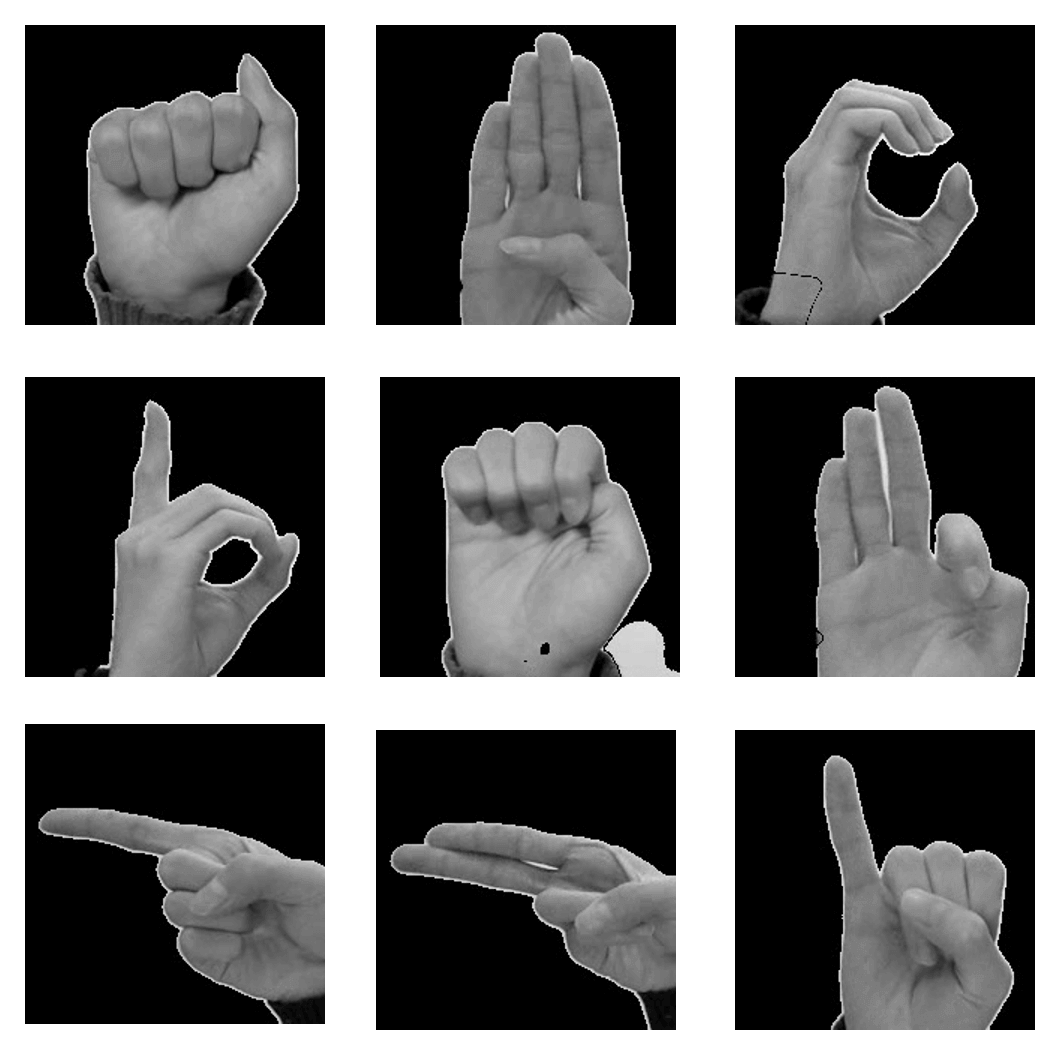
\includegraphics[width=0.9\linewidth]{imgs/dataset.png}
\end{center}
\caption{Samples from custom dataset}
\end{figure}


\end{columns}


\end{frame}

\begin{frame}
\frametitle{Improvement: Average Background Subtraction}

\begin{enumerate}
	\item Running average of first few frames as reference.
	\item Subtract all the subsequent frames with respect to reference.
	\item Pixels that exceed certain threshold are considered to be foreground, while the others are background.
\end{enumerate}

\end{frame}

\begin{frame}
\frametitle{Improvement: Experiment - Accuracy}

\begin{itemize}
	\item Train with the same setting as it is in ASL training.
\end{itemize}

\begin{table}[h]
\begin{center}
\begin{tabular}{|l|c|}
\hline
Dataset & Accuracy \\
\hline\hline
Custom Train & 25804/25809 (100\%) \\
Custom Test & 7364/8700 (85\%) \\
\hline
\end{tabular}
\end{center}
\caption{Results on custom datasets}
\label{table:result}
\end{table}
\end{frame}

\begin{frame}
\frametitle{Preview of Our System}

\begin{figure}
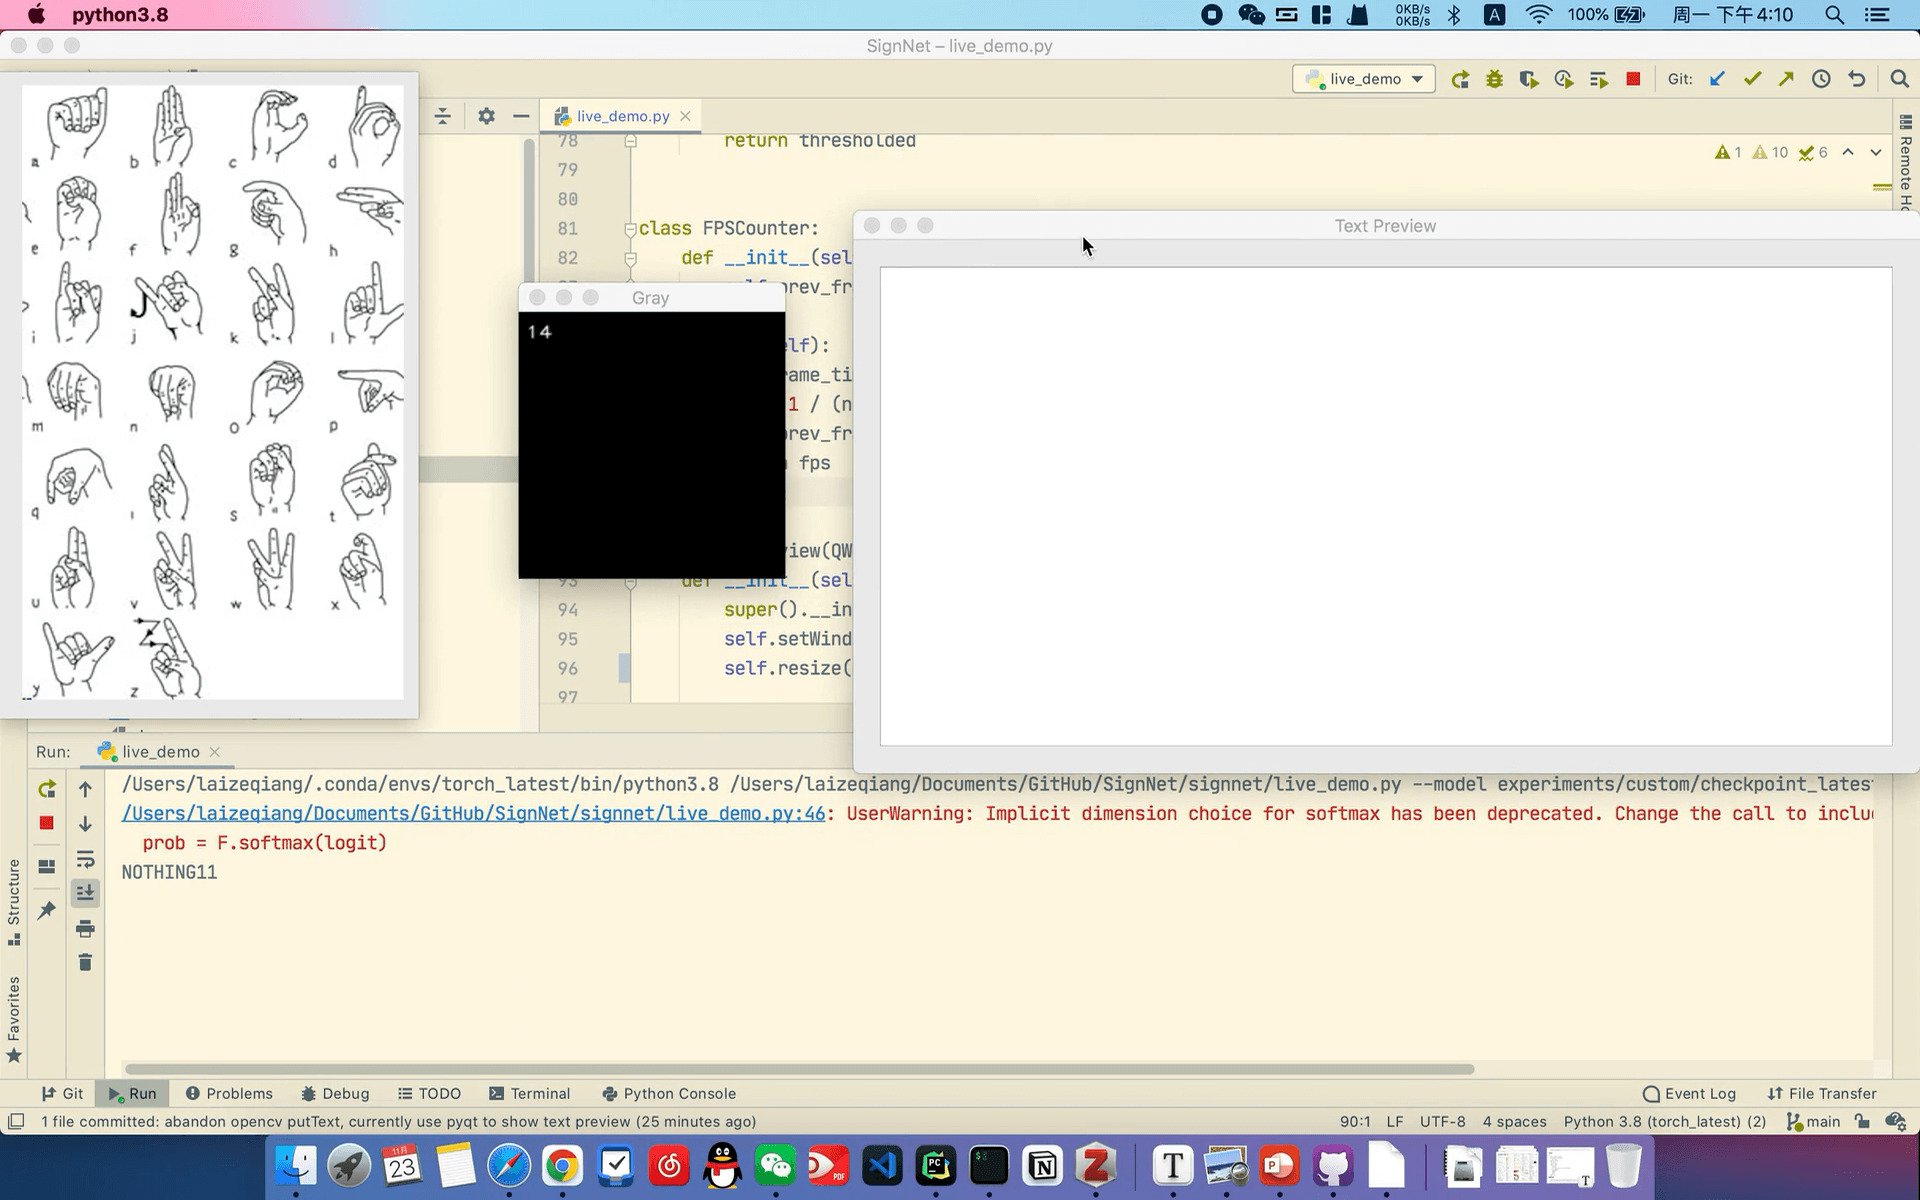
\includegraphics[scale=0.15]{imgs/preview}
\caption{Preview}
\end{figure}

\end{frame}


\begin{frame}
\frametitle{Improvement: Experiment - Confusion}

\begin{figure}[h]
\begin{center}
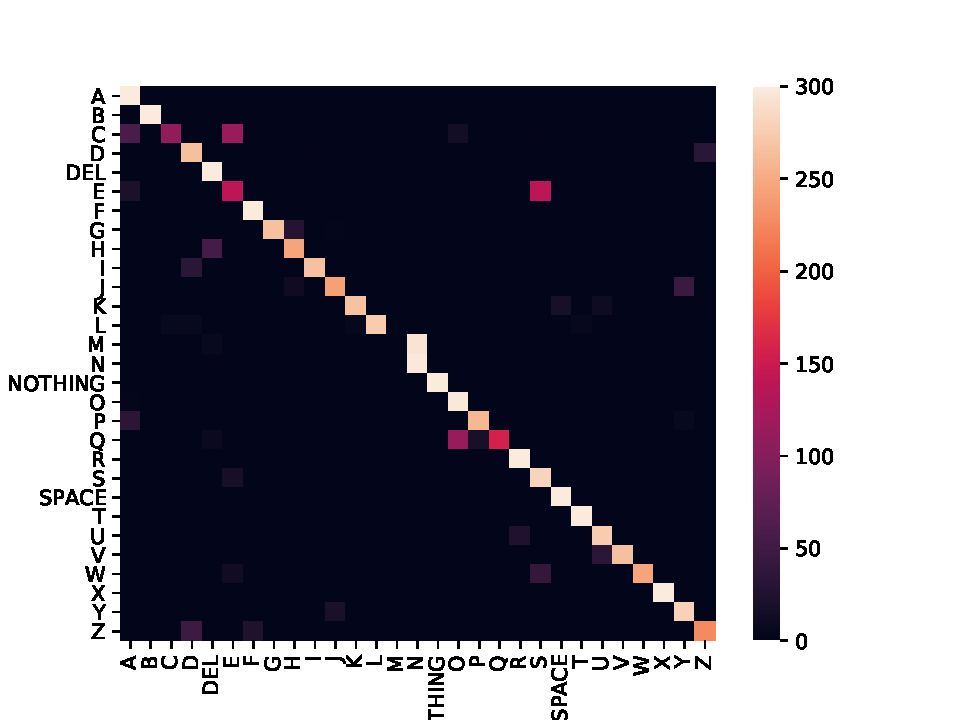
\includegraphics[width=0.7\linewidth]{imgs/confusion}
\end{center}
   \caption{Confusion matrix on custom test set}
\label{fig:confusion}
\end{figure}

\end{frame}

\begin{frame}
\frametitle{Improvement: Experiment - FPS}

\begin{table}[h]
\begin{center}
\begin{tabular}{|l|l|l|l|}
\hline
Hardware              & Platform                & Type   & FPS \\ \hline\hline
\multirow{2}{*}{Intel Core i7}   & \multirow{2}{*}{macOS 10.15.7}  & live   & 15.73  \\ \cline{3-4} 
                      &                         & static & 81.00  \\ \hline
\multirow{2}{*}{Nvidia RTX 2060} & \multirow{2}{*}{Windows 10} & live   & 31.05  \\ \cline{3-4} 
                      &                         & static & 534.12 \\ \hline
Nvidia GTX 1070 & Ubuntu 20.04.1 & static & 453.78 \\ \hline                    
\end{tabular}
\end{center}
\caption{Average FPS of our model in different settings. Type "live" means it is tested using our live\_demo script which uses OpenCV to record video in real time, and type "static" means it is tested using static images.}
\label{table:fps}
\end{table}

\end{frame}

\begin{frame}
\frametitle{Limitations}

\begin{itemize}
	\item Heavily rely on the performance of background subtraction.
	\item Poor performance on some extreme cases.
	\item Sensitive to the size, orientation of gestures. 
\end{itemize}

\end{frame}

\end{document}